\documentclass[9pt,aspectratio=169]{beamer}

\usepackage[utf8]{inputenc}
\usepackage[T1]{fontenc}
\usepackage[english]{babel}
\usepackage{lmodern}
\usepackage{microtype}
\usepackage{amssymb}
\usepackage{listings}
% Shared by report.tex and presentation.tex.
\usepackage{graphicx}
\usepackage{booktabs}
\usepackage{tikz}
\usetikzlibrary{arrows.meta,positioning,fit,calc,shapes.misc}

\definecolor{todored}{HTML}{C0392B}
\definecolor{good}{HTML}{1E8449}
\definecolor{bad}{HTML}{B03A2E}
\definecolor{mesh}{HTML}{2E86C1}

% Anything the team still has to fill in. Search the .tex files for \todo.
\newcommand{\todo}[1]{{\color{todored}\textbf{[TODO:} #1\textbf{]}}}

% \placeholder{width}{height}{text}: red box where a figure will go.
\newcommand{\placeholder}[3]{%
  \fcolorbox{todored}{todored!5}{\parbox[c][#2][c]{\dimexpr#1-2\fboxsep-2\fboxrule\relax}%
    {\centering\color{todored}\small #3}}}

% \evidence{file}{width}{height}{what it should show}
% Shows evidence/<file> once it exists, a placeholder until then.
\newcommand{\evidence}[4]{%
  \IfFileExists{evidence/#1}%
    {\includegraphics[width=#2,height=#3,keepaspectratio]{evidence/#1}}%
    {\placeholder{#2}{#3}{missing \texttt{evidence/#1}\\[2pt]#4}}}

\tikzset{
  >={Stealth},
  svc/.style={draw, rounded corners, minimum width=2.3cm, minimum height=.75cm,
              font=\small\ttfamily, fill=white},
  hacked/.style={svc, draw=bad, fill=bad!12},
  proxy/.style={svc, fill=mesh!15, draw=mesh},
}

\usetikzlibrary{backgrounds}

% Warsaw with the main colour switched to #8B0002 (same as the stage 2 deck)
\usetheme{Warsaw}
\definecolor{MainRed}{HTML}{8B0002}
\definecolor{DarkRed}{HTML}{5A0001}
\definecolor{LightRed}{HTML}{FDF2F2}
\definecolor{AccentGreen}{HTML}{1B5E20}
\definecolor{CodeBg}{HTML}{F7F7F9}

\usecolortheme[named=MainRed]{structure}
\setbeamercolor{alerted text}{fg=MainRed}
\setbeamercolor{example text}{fg=AccentGreen}
\setbeamerfont{section in head/foot}{size=\fontsize{5}{5.7}\selectfont}

% Diagram colours: green = protected by the mesh, red = attacker
\colorlet{mesh}{AccentGreen}
\colorlet{good}{AccentGreen}
\colorlet{bad}{MainRed}
\tikzset{
  svc/.style={draw=DarkRed, thick, rounded corners=3pt, fill=white,
              minimum width=2.1cm, minimum height=.65cm, font=\scriptsize\ttfamily},
  hacked/.style={svc, draw=MainRed, fill=MainRed!15, text=DarkRed},
  proxy/.style={svc, draw=AccentGreen, fill=AccentGreen!10, text=AccentGreen},
  zone/.style={draw=DarkRed!60, thick, dashed, rounded corners=4pt, fill=CodeBg},
  arr/.style={-{Stealth[scale=0.85]}, thick, draw=DarkRed},
  ok/.style={-{Stealth[scale=0.85]}, very thick, draw=AccentGreen},
  no/.style={-{Stealth[scale=0.85]}, thick, dashed, draw=MainRed},
  cross/.style={cross out, draw=MainRed, thick, minimum size=6pt, inner sep=0pt},
}

\lstset{
  language=bash,
  basicstyle=\ttfamily\scriptsize,
  columns=fullflexible,
  keepspaces=true,
  keywordstyle=\color{MainRed}\bfseries,
  commentstyle=\color{gray}\itshape,
  stringstyle=\color{AccentGreen},
  backgroundcolor=\color{CodeBg},
  frame=single,
  rulecolor=\color{MainRed!30},
  showstringspaces=false,
  aboveskip=2pt, belowskip=2pt,
  xleftmargin=3pt, xrightmargin=3pt
}

% Speaker notes: uncomment ONE line below.
% \setbeameroption{show notes on second screen=right}  % slides + notes side by side (pdfpc / dual screen)
% \setbeameroption{show only notes}                    % notes only, printable

\title[Modern Service Mesh -- Stage 3]{\texorpdfstring{Modern Service Mesh -- a better way \\ to secure communication between microservices}{Modern Service Mesh -- a better way to secure communication between microservices}}
\subtitle{Stage 3: Final results}
\author[Bartoszewski, Domagała, Maziarz, Pawłoś]{\texorpdfstring{Jędrzej Bartoszewski \quad Michał Domagała \quad Kacper Maziarz \quad Mikołaj Pawłoś\\[4pt]{\small Selected Issues of Network Applications 2026/2027}}{Bartoszewski, Domagała, Maziarz, Pawłoś}}
\institute[FTIMS PŁ]{\texorpdfstring{Faculty of Technical Physics, Information Technology and Applied Mathematics\\Lodz University of Technology}{FTIMS PŁ}}
\date{November 2026}

\begin{document}

% =============================================================================
% Title
% =============================================================================
\begin{frame}
  \titlepage
\end{frame}
\note{Names and the topic, ten seconds, move on.}

% =============================================================================
\section{Problem}
% =============================================================================

\begin{frame}{Inside the cluster, everyone trusts everyone}
  \begin{columns}[T,onlytextwidth]
    \begin{column}{0.42\textwidth}
      \begin{block}{Kubernetes by default}
        \begin{itemize}\setlength{\itemsep}{3pt}
          \item Online Boutique: 11 services talking gRPC and HTTP, all \alert{plaintext}
          \item Any pod can call any other pod; nobody checks who's asking
          \item Firewalls guard the edge (North-South); East-West traffic inside the cluster gets no checks at all
        \end{itemize}
      \end{block}
    \end{column}
    \begin{column}{0.55\textwidth}
      \centering
      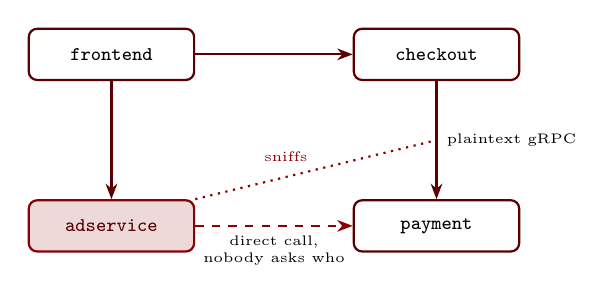
\begin{tikzpicture}[node distance=.6cm and 2.0cm]
        \node[svc]                 (fe)  {frontend};
        \node[svc, right=of fe]    (co)  {checkout};
        \node[svc, below=1.5cm of co] (pay) {payment};
        \node[hacked, below=1.5cm of fe] (ad) {adservice};
        \draw[arr] (fe) -- (co);
        \draw[arr] (co) -- node[right, font=\tiny]{plaintext gRPC} (pay);
        \draw[arr] (fe) -- (ad);
        \draw[no] (ad) -- node[below, font=\tiny, align=center]{direct call,\\nobody asks who} (pay);
        \draw[MainRed, thick, dotted] (ad.north east) -- node[above left=-1pt, font=\tiny]{sniffs} ($(co)!.5!(pay)$);
      \end{tikzpicture}
    \end{column}
  \end{columns}
\end{frame}
\note{The scenario the whole project is built around. An attacker who gets
into one small service, here the ad service, can read the traffic passing by
and call the payment service directly, because nothing checks who is calling.}

\begin{frame}{Three gaps, three fixes}
  \centering
  \vspace{4pt}
  \begin{tabular}{llll}
    \toprule
    \textbf{Attack}  & \textbf{Gap} & \textbf{Fix} & \textbf{Closed in} \\
    \midrule
    Eavesdropping    & plaintext traffic                 & mutual TLS                   & step 2 \\
    Impersonation    & no cryptographic identity         & a certificate per service    & step 2 \\
    Lateral movement & nothing restricts who calls whom  & \textbf{authorization policies} & \textbf{step 3} \\
    \bottomrule
  \end{tabular}

  \vspace{12pt}
  \begin{alertblock}{Where stage 2 ended}
    Every connection encrypted, every service with its own identity, and still
    any pod could call \texttt{paymentservice}. Encrypted $\neq$ protected.
  \end{alertblock}
\end{frame}
\note{Three separate problems that need separate fixes. After stage 2 the first
two were closed, but the third was wide open: two test pods, one outside the
mesh and one with the ad service's identity, both reached payment and cart.
This stage closes the third gap and shows it.}

% =============================================================================
\section{Idea}
% =============================================================================

\begin{frame}{Our idea: Zero Trust, enforced by the infrastructure}
  \begin{block}{Service mesh}
    \begin{itemize}\setlength{\itemsep}{2pt}
      \item A small proxy next to every service handles all of its traffic
      \item Proxies encrypt with mutual TLS and prove identity with certificates
      \item Policies decide which identity may call which method
      \item \textbf{No change to application code}
    \end{itemize}
  \end{block}
  \vfill
  \centering
  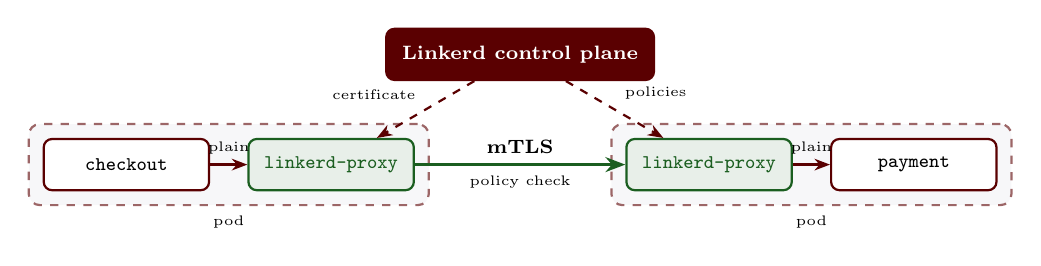
\begin{tikzpicture}[font=\scriptsize]
    \node[svc]   (a1) at (0,0)    {checkout};
    \node[proxy] (p1) at (2.6,0)  {linkerd-proxy};
    \node[proxy] (p2) at (7.4,0)  {linkerd-proxy};
    \node[svc]   (a2) at (10.0,0) {payment};
    \begin{scope}[on background layer]
      \node[zone, fit=(a1)(p1), inner sep=5pt, label={[font=\tiny]below:pod}] {};
      \node[zone, fit=(a2)(p2), inner sep=5pt, label={[font=\tiny]below:pod}] {};
    \end{scope}
    \draw[arr] (a1) -- node[above, font=\tiny]{plain} (p1);
    \draw[ok] (p1) -- node[above]{\textbf{mTLS}} node[below, font=\tiny]{policy check} (p2);
    \draw[arr] (p2) -- node[above, font=\tiny]{plain} (a2);
    \node[svc, fill=DarkRed, text=white, minimum width=3.4cm, font=\scriptsize\bfseries] (cp) at (5,1.4) {Linkerd control plane};
    \draw[arr, dashed] (cp) -- node[above left, font=\tiny]{certificate} (p1);
    \draw[arr, dashed] (cp) -- node[above right, font=\tiny]{policies} (p2);
  \end{tikzpicture}
\end{frame}
\note{The original idea from stage 1, unchanged: put the security in the
infrastructure instead of the five languages the shop is written in. The
receiving proxy knows the caller's identity from its certificate, so it can
decide per request whether that identity may call that method.}

\begin{frame}{The stack}
  \begin{columns}[T,onlytextwidth]
    \begin{column}{0.42\textwidth}
      \begin{block}{Tools (versions pinned by the scripts)}
        \begin{itemize}\setlength{\itemsep}{3pt}
          \item \textbf{k3d v5.9.0:} Kubernetes in Docker, one server and two agents
          \item \textbf{Online Boutique v0.10.7:} the shop we attack
          \item \textbf{Linkerd edge-26.11.1:} mTLS, identity, authorization policies
          \item \textbf{Prometheus (linkerd-viz) + Grafana 11.3.0:} allowed vs.\ denied traffic
        \end{itemize}
      \end{block}
    \end{column}
    \begin{column}{0.55\textwidth}
      \centering
      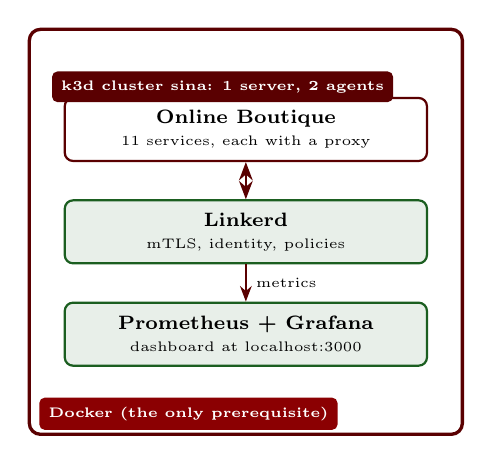
\begin{tikzpicture}[font=\scriptsize,
          box/.style={svc, font=\scriptsize, align=center, minimum width=4.6cm, minimum height=.8cm}]
        \node[box]                                        (ob)  at (0,0)    {\textbf{Online Boutique}\\\tiny 11 services, each with a proxy};
        \node[box, draw=AccentGreen, fill=AccentGreen!10] (l5d) at (0,-1.3) {\textbf{Linkerd}\\\tiny mTLS, identity, policies};
        \node[box, draw=AccentGreen, fill=AccentGreen!10] (mon) at (0,-2.6) {\textbf{Prometheus + Grafana}\\\tiny dashboard at localhost:3000};
        \draw[arr, <->] (ob) -- (l5d);
        \draw[arr] (l5d) -- node[right, font=\tiny]{metrics} (mon);
        \begin{scope}[on background layer]
          \node[zone, fit=(ob)(l5d)(mon), inner sep=8pt, inner ysep=12pt] (k3d) {};
          \node[draw=DarkRed, very thick, rounded corners=4pt, fill=white, fit=(k3d), inner sep=4pt, inner ysep=12pt] (dock) {};
        \end{scope}
        \node[fill=DarkRed, text=white, font=\tiny\bfseries, rounded corners=2pt, anchor=north west]
          at ([xshift=4pt,yshift=-3pt]k3d.north west) {k3d cluster sina: 1 server, 2 agents};
        \node[fill=MainRed, text=white, font=\tiny\bfseries, rounded corners=2pt, anchor=south west]
          at ([xshift=4pt,yshift=2pt]dock.south west) {Docker (the only prerequisite)};
      \end{tikzpicture}
    \end{column}
  \end{columns}
\end{frame}
\note{Everything comes up with one script, setup.sh or setup.ps1. Docker is the
only prerequisite; the script downloads pinned versions of the tools.
Compared with stage 2, the monitoring layer at the bottom is now real.}

% =============================================================================
\section{Solution}
% =============================================================================

\begin{frame}{All five steps delivered}
  \centering
  \vspace{4pt}
  \begin{tabular}{llll}
    \toprule
    \textbf{Step} & \textbf{When} & \textbf{Owner} & \textbf{Status} \\
    \midrule
    1. k3d cluster + Online Boutique      & weeks 3--4         & Mikołaj  & \textcolor{AccentGreen}{\textbf{done}} \\
    2. Linkerd + mTLS proof of concept    & weeks 5--6 (6.11)  & Jędrzej  & \textcolor{AccentGreen}{\textbf{done}} \\
    3. Zero-Trust authorization policies  & week 7             & Michał   & \textcolor{AccentGreen}{\textbf{done}} \\
    4. Prometheus + Grafana               & week 8             & Kacper   & \textcolor{AccentGreen}{\textbf{done}} \\
    5. Attack simulation                  & week 9 (27.11)     & Michał   & \textcolor{AccentGreen}{\textbf{done}} \\
    \bottomrule
  \end{tabular}

  \vspace{10pt}
  {\small \texttt{./setup.sh}: the ``before'' cluster \quad$\cdot$\quad
  \texttt{./setup.sh -{}-protect}: everything on\\[2pt]
  \texttt{./zero-trust.sh on|off}: switch the policies in seconds, no restarts}
\end{frame}
\note{The schedule from stage 1, all done. The bottom line is how the result is
used: the same script builds the unprotected or the protected cluster, and
zero-trust.sh switches the policies on a running cluster without restarting a
single pod, which is what the live demo relies on.}

\begin{frame}{Step 3: who may call what}
  \begin{columns}[T,onlytextwidth]
    \begin{column}{0.46\textwidth}
      \begin{block}{Allow-matrix from real traffic}
        \begin{itemize}\setlength{\itemsep}{2pt}
          \item Recorded with \texttt{linkerd viz tap}: loadgenerator traffic + orders by hand
          \item 14 gRPC connections $\to$ 20 (caller, method) pairs
          \item Caller = Kubernetes ServiceAccount = mTLS identity
          \item Per \textbf{method}, not per port: frontend may get a shipping quote, but not ship an order
        \end{itemize}
      \end{block}
    \end{column}
    \begin{column}{0.52\textwidth}
      \centering
      {\scriptsize
      \begin{tabular}{lll}
        \toprule
        \textbf{Service} & \textbf{Method} & \textbf{Callers} \\
        \midrule
        payment  & \texttt{Charge}                & checkout \\
        email    & \texttt{SendOrderConfirmation} & checkout \\
        checkout & \texttt{PlaceOrder}            & frontend \\
        cart     & \texttt{GetCart}, \texttt{EmptyCart} & frontend, checkout \\
                 & \texttt{AddItem}               & frontend \\
        shipping & \texttt{GetQuote}              & frontend, checkout \\
                 & \texttt{ShipOrder}             & checkout \\
        catalog  & \texttt{SearchProducts}        & \alert{nobody} \\
        \multicolumn{3}{l}{\tiny \ldots{} 6 more rows; health checks: kubelet by node address} \\
        \bottomrule
      \end{tabular}}
    \end{column}
  \end{columns}
\end{frame}
\note{Before writing a single rule we recorded what the shop really does. The
result is the allow-matrix: for every service, which methods exist and which
identities call them. Anything not in the matrix is refused. SearchProducts is
part of the API, but nothing in the shop calls it, so nobody may.}

\begin{frame}{Step 3: how a rule looks in Linkerd}
  \centering
  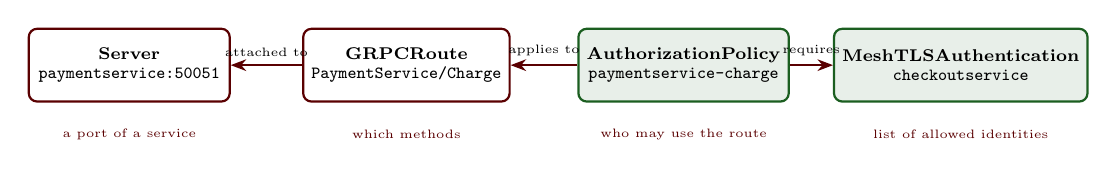
\begin{tikzpicture}[font=\scriptsize, scale=0.88, transform shape,
      res/.style={svc, align=center, minimum width=2.9cm, minimum height=1.05cm, font=\scriptsize}]
    \node[res]                                         (srv) at (0,0)    {\textbf{Server}\\\ttfamily paymentservice:50051};
    \node[res]                                         (rt)  at (4,0)    {\textbf{GRPCRoute}\\\ttfamily PaymentService/Charge};
    \node[res, draw=AccentGreen, fill=AccentGreen!10]  (ap)  at (8,0)    {\textbf{AuthorizationPolicy}\\\ttfamily paymentservice-charge};
    \node[res, draw=AccentGreen, fill=AccentGreen!10]  (mt)  at (12,0)   {\textbf{MeshTLSAuthentication}\\\ttfamily checkoutservice};
    \draw[arr] (rt) -- node[above, font=\tiny]{attached to} (srv);
    \draw[arr] (ap) -- node[above, font=\tiny]{applies to} (rt);
    \draw[arr] (ap) -- node[above, font=\tiny]{requires} (mt);
    \node[font=\tiny, align=center, text=DarkRed] at (0,-1)  {a port of a service};
    \node[font=\tiny, align=center, text=DarkRed] at (4,-1)  {which methods};
    \node[font=\tiny, align=center, text=DarkRed] at (8,-1)  {who may use the route};
    \node[font=\tiny, align=center, text=DarkRed] at (12,-1) {list of allowed identities};
  \end{tikzpicture}

  \vspace{14pt}
  \begin{columns}[T,onlytextwidth]
    \begin{column}{0.48\textwidth}
      \begin{block}{In \texttt{policies/}}
        11 \texttt{Server}s, 22 \texttt{GRPCRoute}s, 25 \texttt{AuthorizationPolicy}
        objects, 7 shared authentications. \texttt{frontend} and \texttt{redis-cart}:
        per port.
      \end{block}
    \end{column}
    \begin{column}{0.48\textwidth}
      \begin{exampleblock}{Rollout}
        Audit mode first: the proxy only records what it would deny. On the
        gRPC services only attacker pods showed up, so we switched to enforcing.
      \end{exampleblock}
    \end{column}
  \end{columns}
\end{frame}
\note{One rule is four small Kubernetes resources: the Server picks the port,
the route picks the methods, the policy says who may use the route by pointing
to a list of identities. A request gets through only if it matches a route and
passes that route's policy. Before enforcing, we ran everything in audit mode
to make sure no legitimate call would be blocked.}

\begin{frame}{Step 3: what the attackers can still do}
  \newcommand{\yes}{\textcolor{AccentGreen}{\large$\checkmark$}}
  \newcommand{\nope}{\textcolor{MainRed}{\large$\times$}}
  \centering
  {\small
  \begin{tabular}{lcccc}
    \toprule
    \textbf{Attacker pod} & \texttt{Charge} & \texttt{SendOrderConfirmation} & \texttt{ShipOrder} & \texttt{GetQuote} \\
                          & \scriptsize payment & \scriptsize email & \scriptsize shipping & \scriptsize shipping \\
    \midrule
    outside the mesh       & \nope & \nope & \nope & \nope \\
    as \texttt{adservice} & \nope & \nope & \nope & \nope \\
    as \texttt{frontend}  & \nope & \nope & \nope & \yes \\
    \bottomrule
  \end{tabular}}

  \vspace{2pt}
  {\tiny The outside and adservice pods are refused on all 14 methods of the matrix, not only these four.}

  \vspace{8pt}
  \begin{columns}[T,onlytextwidth]
    \begin{column}{0.48\textwidth}
      \begin{block}{Three test pods}
        \begin{itemize}\setlength{\itemsep}{2pt}
          \item \textbf{Outside the mesh} and \textbf{as adservice}: every method refused
          \item \textbf{As frontend}: keeps the frontend's own rights, nothing more
        \end{itemize}
      \end{block}
    \end{column}
    \begin{column}{0.48\textwidth}
      \begin{alertblock}{Least privilege limits the damage}
        A hijacked frontend can still ask for a shipping quote, as the real one
        must, but can't charge a card or ship an order.
      \end{alertblock}
    \end{column}
  \end{columns}
\end{frame}
\note{Three attacker pods. The one outside the mesh and the one with the ad
service's identity are refused everywhere. The interesting one runs as the
frontend: it can still do what the frontend legitimately does, like asking for
a shipping quote, but it can no longer charge a card, send an email or ship an
order. Kubernetes NetworkPolicy can't express this, because it works on IP
addresses and doesn't see gRPC methods.}

\begin{frame}{Step 3: verified in 47 cases}
  \begin{columns}[T,onlytextwidth]
    \begin{column}{0.58\textwidth}
      {\scriptsize
      \begin{tabular}{p{5.0cm}rl}
        \toprule
        \textbf{\texttt{attack/verify.sh}} & & \textbf{Policies on} \\
        \midrule
        every method, outside + adservice pods     & 28 & denied (7) \\
        Charge, ShipOrder, SendOrder\ldots{} as frontend & 3 & denied \\
        GetQuote as frontend                       & 1 & reaches app \\
        SearchProducts, all three pods             & 3 & no route (5) \\
        health check, all three pods               & 3 & denied \\
        Redis \texttt{PING}, all three pods        & 3 & no answer \\
        shop: home, add to cart, checkout          & 3 & order confirmed \\
        pods 2/2, no restarts, no legit denials    & 3 & as expected \\
        \midrule
        total                                      & 47 & \textcolor{AccentGreen}{\textbf{all passed}} \\
        \bottomrule
      \end{tabular}}
    \end{column}
    \begin{column}{0.38\textwidth}
      \begin{block}{gRPC status}
        \begin{itemize}\setlength{\itemsep}{1pt}
          \item 0, 2: reached the application
          \item 7 \texttt{PERMISSION\_DENIED}: stopped by the proxy
          \item 5 \texttt{NOT\_FOUND}: no route
        \end{itemize}
      \end{block}
      \begin{exampleblock}{Before the policies}
        \texttt{verify.sh -{}-expect-open}: every attack case reaches the application.
      \end{exampleblock}
    \end{column}
  \end{columns}
\end{frame}
\note{The test script checks the whole matrix from the three attacker pods, and
also that the shop still works and that no legitimate caller was refused. We
first wrote a version that could pass on a broken setup, for example it took a
missing route for success, so we broke the cluster on purpose for each case
until the script caught it.}

\begin{frame}[fragile]{Step 3: closing the last open port}
  \begin{columns}[T,onlytextwidth]
    \begin{column}{0.50\textwidth}
      \begin{block}{Namespace default-deny}
        \begin{itemize}\setlength{\itemsep}{2pt}
          \item A port without a \texttt{Server} falls back to \texttt{all-unauthenticated}
          \item In practice: the proxy admin port 4191, which exposes every service's metrics
          \item Default \texttt{deny} for the namespace: only Prometheus may read \texttt{/metrics}, only the kubelet the health checks
        \end{itemize}
      \end{block}
    \end{column}
    \begin{column}{0.46\textwidth}
\begin{lstlisting}[language={}, basicstyle=\ttfamily\fontsize{6}{7.2}\selectfont]
$ curl http://<paymentservice>:4191/metrics
attacker-outside       -> 403
attacker-as-adservice  -> 403
attacker-as-frontend   -> 403
\end{lstlisting}
      \begin{exampleblock}{Part of \texttt{setup.sh -{}-protect}}
        Set before the shop starts, so no pod restarts. On a running cluster
        switching it restarts every pod.
      \end{exampleblock}
    \end{column}
  \end{columns}
\end{frame}
\note{The per-service policies cover every application port, but the proxy's
own admin port stayed open, so any pod could read another service's traffic
metrics. The namespace default-deny closes it. The protected setup turns it on
before the shop starts. For the live demo we use a cluster without it, because
switching it on a running cluster restarts every pod.}

\begin{frame}{Step 4: the denials on a dashboard}
  \centering
  \evidence{10-grafana.png}{0.86\textwidth}{5.6cm}{Grafana dashboard after the attack}

  \vspace{3pt}
  {\scriptsize Grafana on the linkerd-viz Prometheus: 16 denied calls, each with the target, the method and the caller's identity}
\end{frame}
\note{Kacper. Grafana reads the Prometheus that comes with linkerd-viz, which
already scrapes every proxy. The top row: denied calls, allowed requests,
share of calls with a verified identity, denied TCP and denied health checks,
which must stay at zero. The table at the bottom says who was refused where:
the ad service identity and the pod outside the mesh. One surprise: Grafana
itself got 403 from Prometheus until it was meshed and given its own policy.}

\begin{frame}[fragile]{Step 5: the same attack, before and after}
\begin{lstlisting}[language={}, morecomment={[l]{\#}}, basicstyle=\ttfamily\fontsize{6}{7.4}\selectfont]
# ./zero-trust.sh off   (mTLS only, like stage 2)
$ attack/attack.sh
attacker-outside       -> paymentservice  Charge   grpc-status: 2  Cannot read ... (reading 'credit_card_number')
attacker-outside       -> cartservice     GetCart  grpc-status: 0
attacker-as-adservice  -> paymentservice  Charge   grpc-status: 2  Cannot read ... (reading 'credit_card_number')
attacker-as-adservice  -> cartservice     GetCart  grpc-status: 0
\end{lstlisting}
\vspace{4pt}
\begin{lstlisting}[language={}, morecomment={[l]{\#}}, basicstyle=\ttfamily\fontsize{6}{7.4}\selectfont]
# ./zero-trust.sh on    (authorization policies)
$ attack/attack.sh
attacker-outside       -> paymentservice  Charge   grpc-status: 7
attacker-outside       -> cartservice     GetCart  grpc-status: 7
attacker-as-adservice  -> paymentservice  Charge   grpc-status: 7  unauthorized request on route
attacker-as-adservice  -> cartservice     GetCart  grpc-status: 7  unauthorized request on route
\end{lstlisting}
  \vspace{6pt}
  \centering
  {\small Before: the payment service itself answers (it only fails on the missing card data).
  After: \alert{\texttt{PERMISSION\_DENIED}} from the proxy; the request never reaches the application.}
\end{frame}
\note{Michał. The attack from stage 2, unchanged. Without policies, Charge comes
back with the payment service's own error about the missing card number: the
call got all the way into the application. With the policies, every call ends
with status 7 at the proxy. Output shortened; the report has all four calls
in a table.}

\begin{frame}{What it costs}
  \centering
  {\small
  \begin{tabular}{lrrr}
    \toprule
    \textbf{Median latency at 20 req/s} & \textbf{No mesh} & \textbf{mTLS} & \textbf{mTLS + policies} \\
    \midrule
    \texttt{ListProducts}, direct gRPC & 0.8 ms  & 1.7 ms  & 1.7 ms \\
    product page                       & 10.9 ms & 22.7 ms & 22.6 ms \\
    home page                          & 16.4 ms & 28.3 ms & 27.4 ms \\
    \bottomrule
  \end{tabular}}

  \vspace{10pt}
  \begin{columns}[T,onlytextwidth]
    \begin{column}{0.48\textwidth}
      \begin{block}{Mesh: proxies + mTLS}
        About +1 ms per hop, +12 ms on a page that makes many calls. Page
        throughput unchanged (45--58 req/s, limited by the shop's CPU limits).
      \end{block}
    \end{column}
    \begin{column}{0.48\textwidth}
      \begin{exampleblock}{Policies}
        No measurable cost: medians differ by less than 1 ms. Proxies: about
        3.6 MiB each after start, 280 millicores together at 20 req/s.
      \end{exampleblock}
    \end{column}
  \end{columns}

  \vspace{4pt}
  {\tiny fortio, median of 3 runs of 60 s per variant, one laptop: only for comparing the variants}
\end{frame}
\note{Kacper measured it. The mesh is what costs, the proxies with mTLS between
them: roughly one millisecond per call between services. We did not measure the
encryption on its own. The authorization check on top is free within the
precision of a laptop measurement.}

\begin{frame}{What we learned}
  \vfill
  \begin{columns}[T,onlytextwidth]
    \begin{column}{0.465\textwidth}
      \begin{block}{Policies}
        \begin{itemize}\setlength{\itemsep}{9pt}
          \item Once a port has a policy, every request needs a route, so per-method rules cost little extra
          \item Health checks come from the kubelet, which has no identity: allowed by node address
          \item An empty \texttt{ShipOrder} crashes \texttt{shippingservice}; without policies any pod can restart it
        \end{itemize}
      \end{block}
    \end{column}
    \begin{column}{0.465\textwidth}
      \begin{block}{Running it}
        \begin{itemize}\setlength{\itemsep}{9pt}
          \item Our first test script passed on a broken setup; we broke the cluster on purpose to fix it
          \item Monitoring needs its own authorization: Grafana got 403 from Prometheus
          \item 6--7 GB for Docker; an overloaded cluster starts pods without a proxy, and the policies treat them as outsiders
        \end{itemize}
      \end{block}
    \end{column}
  \end{columns}
  \vfill
\end{frame}
\note{Pick two or three of these depending on time. The ShipOrder crash is a
good one: the policies also protect the application from its own bugs, because
only checkout may send that request at all.}

% =============================================================================
\section{Further development}
% =============================================================================

\begin{frame}{Limits and what could come next}
  \vfill
  \begin{columns}[T,onlytextwidth]
    \begin{column}{0.465\textwidth}
      \begin{alertblock}{Limits}
        \begin{itemize}\setlength{\itemsep}{9pt}
          \item Health-check rules tied to our three nodes
          \item A hijacked service keeps its own rights
          \item linkerd-viz Prometheus keeps 6 hours of data
          \item Tested on one Linkerd edge release only
        \end{itemize}
      \end{alertblock}
    \end{column}
    \begin{column}{0.465\textwidth}
      \begin{exampleblock}{Further development}
        \begin{itemize}\setlength{\itemsep}{9pt}
          \item Separate Prometheus with long retention and alerts on denials
          \item Health-check rules that don't depend on node addresses
          \item \texttt{verify.sh} run automatically after every policy change
          \item Policies generated from observed traffic instead of by hand
        \end{itemize}
      \end{exampleblock}
    \end{column}
  \end{columns}
  \vfill
\end{frame}
\note{The limits are the honest list from the report. The last extension is the
natural next step for a bigger system: we built the allow-matrix by watching
the traffic, and that could be automated.}

% =============================================================================
\section{Demo}
% =============================================================================

\begin{frame}
  \centering
  \vspace{1.2cm}
  \begin{beamercolorbox}[sep=14pt,center,shadow=true,rounded=true]{title}
    {\LARGE \textbf{Live demo}}
  \end{beamercolorbox}
\end{frame}
\note{Switch to the laptop with the cluster. Prepare it before the
presentation with ./setup.sh (no --protect), so on/off take seconds.
(1) ./zero-trust.sh status; (2) ./zero-trust.sh off, attack/attack.sh: the
calls reach the application (status 2 and 0); (3) ./zero-trust.sh on,
attack/attack.sh two or three times about 15 s apart: status 7, the first
denial of a new caller doesn't show on the per-second chart; (4) Grafana at
localhost:3000: who was denied; (5) the shop at localhost:8080 still takes an
order. If anything fails, go back to the Step 4 and Step 5 slides, which show
the same output. Then questions.}

\end{document}
